\section{Applications to crystallography}
The notion of form in crystallography can be clarified using the concept of orbits. The ordinary salt forms cubic crystals if it is allowed to crystallize under controlled suitable conditions. We can consider the cube as its in $\mathbb{R}^3$ denoted by C, with its vertices at $(\pm1, \pm1,\pm1)$. Let the group of all orthogonal transformation which carry C into itself be denoted by $O_{h}$. The only linear transformations that preserve the cube are the ones that takes the $(x,y,z)$ to $(u,v,w)$ where u,v,w are the permutations of $\pm x,\pm y, \pm z$. Now $\pm$ can be distributed to x,y or z. So there are $2^3$ choices of $\pm$ and there are $3!$ ways of permuting the x.y and z. So, the total number of elements in $O_{h}$ is $2^3 \times 3!=48 $.

Now if we add urea to the NaCl crystals, then at the corners of the cube, small equilateral congruent triangle starts to form. Since the triangles are congruent, the crystal is still invariant under $O_h$. As the amount of urea increases, the size of the triangles increases and the faces become hexagons, and finally it becomes an octahedron. The group preserving the octahedron is same as the one preserving the cube hence the name $O_{h}$. 

In order to get the cubic crystals, one has to make it in carefully controlled conditions. Normally formed crystals are irregular in shape but in some sense it exhibits symmetry. The transition of the cube as the amount of urea increases in shown in figure 1 a$\longrightarrow$d. But the angles between the corresponding sides of all the crystals Will be same as its given by Nicolas steno and Christian Huygens as the "Law of corresponding angles".

\begin{figure}[H]
    \centering
    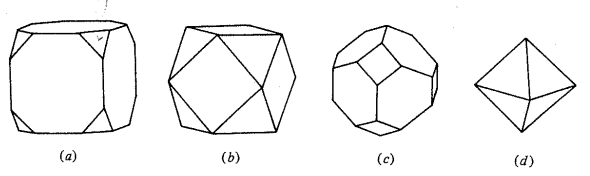
\includegraphics[width = 7.5cm]{fig1.png}
    \caption{Action of urea on the NaCl crystal~\cite{sternberg1995group}}
    \label{fig1}
\end{figure}

We can better understand what crystallographers mean when they talk about a crystal's "shape" by using the concept of an orbit of a group action. The observable symmetry of a crystal is best described in terms of directions, as we have already stated. The collection of normal directions to the faces, according to the law of the constancy of matching angles, is what is invariant (up to an overall rotation). Even though the crystal may have a somewhat uneven exterior, these instructions apply to all crystals of the same composition. These directions can be thought of as points on the unit sphere. This collection of points is affected by the crystal's group of symmetries. \textit{An orbit of the symmetry group acting on this set of directions is what is called a form of the crystal}